\documentclass[10pt]{article}
\usepackage[margin=0.78in]{geometry}
\usepackage{amsmath,amssymb,amsthm,bm,booktabs,graphicx,microtype}
\usepackage{hyperref,xcolor}
\usepackage[numbers,sort&compress]{natbib}
\newtheorem{proposition}{Proposition}
\newtheorem{theorem}{Theorem}
\newtheorem{remark}{Remark}
\DeclareMathOperator{\softmax}{softmax}
\DeclareMathOperator{\tr}{tr}
\title{Posterior-Moment In-Context Solvers for Bayesian Near-Field Linear Sampling}
\author{Technical results note}
\date{4 August 2026}
\begin{document}
\maketitle

\begin{abstract}
We formulate the original two-dimensional near-field linear sampling method
(LSM) as a kernel Bayesian inverse problem and adapt the parallel posterior-
predictive recurrences of Kang, Lee and Cheng to this setting.  Point sources
illuminate one to six sound-soft obstacles and a distinct receiver array records
the complex scattered near field.  A prescribed von Mises/softmax covariance is
a modelling choice: neither its nonlinearity nor a temperature is learned.  A
single tied loop solves both the probe equation, which determines the posterior
mean, and the matrix equation required for posterior covariance.  Richardson,
heavy-ball (HB), Chebyshev and PCG cells therefore share the same encoder,
decoder and Bayesian semantics.  We prove the corresponding depth laws and
show that learned population whitening accelerates ordinary CG substantially,
while it cannot remove all obstacle-dependent eigendirections.  A controlled
multi-obstacle audit reports localization,
residual, calibration and robustness.  Its main negative result is useful:
finite-horizon HB benefits from deliberately conservative effective endpoints,
whereas plugging in the exact spectral endpoints produces a large transient.
Small residuals require either substantially greater depth or adaptive Krylov
coefficients.
\end{abstract}

\section{Scope and correction of the problem}
This note concerns deterministic active \emph{near-field} LSM, not scalar
one-dimensional Gaussian-process regression, not a Born far-field surrogate,
and not the random-source LSM variants of \citet{montanelli2022,montanelli2024}.
For each task, source and receiver locations lie on separate circles.  The
measured object is the full multistatic near-field matrix $N_D$ generated by a
sound-soft obstacle $D$.  The random objects in training are obstacles,
acquisition perturbations and additive noise; the incident point sources are
controlled and deterministic.

\section{Physical near-field model}
Let $\Gamma_s=\{y_j\}_{j=1}^{n_s}$ and
$\Gamma_r=\{x_i\}_{i=1}^{n_r}$ denote source and receiver curves.  With
$\Phi_k(x,y)=\tfrac{\mathrm i}{4}H_0^{(1)}(k|x-y|)$, the incident field
from $y_j$ is $u_j^i(x)=\Phi_k(x,y_j)$.  For a sound-soft obstacle,
\[
 (\Delta+k^2)u_j^s=0\quad\text{outside }D,
 \qquad u_j^s=-u_j^i\quad\text{on }\partial D,
\]
together with the Sommerfeld radiation condition.  The data matrix is
$(N_D)_{ij}=u_j^s(x_i)$.  Numerical data are generated by boundary
collocation with interior fundamental sources; the mean relative boundary
residual in the audit is 2.41e-06.  This is an independent sound-soft
forward model, not reused code from \texttt{lsmlab}.

For every sampling point $z$ in a two-dimensional grid, define
$\phi_z=(\Phi_k(x_i,z))_i$.  After whitening the known receiver-noise
covariance $R_\Gamma$, we retain the same symbols for
$R_\Gamma^{-1/2}N_D$ and $R_\Gamma^{-1/2}\phi_z$.  This is the original
near-field sampling equation $N_Dg_z\simeq\phi_z$ in a statistically explicit
form.

\section{A fixed nonlinear feature model}
For source angles $\theta_i$, let
\[
 W_{ij}=\exp\!\left[\gamma\cos(\theta_i-\theta_j)\right],\qquad
 K_\Gamma=(1-\eta)I+\eta D_W^{-1/2}WD_W^{-1/2}.
\]
This is the symmetric positive version of row-softmax attention.  In the
reported model $\gamma=1.0$ and
$\eta=0.2$ are fixed before training.  The softmax
nonlinearity selects the GP feature space; it is not an optimizable temperature.
Other prior knowledge can be encoded by replacing $\cos(\theta_i-\theta_j)$
with a task-appropriate feature similarity while preserving positive
definiteness.

The proper-complex prior is $g\sim\mathcal{CN}(0,K_\Gamma)$ and whitened
noise has identity covariance.  Set
\[
 H_D=N_DK_\Gamma N_D^*+I.
\]
For the matrix $\Phi=[\phi_z]_z$, the two posterior equations are
\begin{equation}\label{eq:two-solves}
 H_DQ_\mu=\Phi,
 \qquad H_DQ_\Sigma=N_DK_\Gamma.
\end{equation}

\begin{proposition}[Parallel posterior moments]\label{prop:moments}
The conditional coefficient field associated with the probe matrix has mean
and covariance
\[
 M_D=K_\Gamma N_D^*Q_\mu,
 \qquad
 \Sigma_D=K_\Gamma-K_\Gamma N_D^*Q_\Sigma.
\]
Consequently, applying one tied linear recurrence to the concatenated right-
hand side $[\Phi,N_DK_\Gamma]$ computes both posterior moments with identical
solver coefficients and depth.
\end{proposition}
\begin{proof}
These are the Woodbury-form conditioning identities for a linear proper-
complex Gaussian model.  Both expressions contain the same inverse $H_D^{-1}$,
which proves the shared recurrence statement.
\end{proof}

This is the exact near-field analogue of the two parallel recurrences used for
posterior predictive mean and variance in \citet{kang2026}.  It also clarifies
terminology: the matrices $B^*A^jB$ used below are \emph{spectral Krylov
statistics} for the controller, not posterior moments.

\section{Architecture}
Let $C_{\mathrm{pop},\Gamma}$ be a geometry-conditioned factor diagonal in
the prescribed receiver-feature basis.  The task supplies
\[
 A_D=s_D^{-1}C_{\mathrm{pop},\Gamma}^*H_D
 C_{\mathrm{pop},\Gamma},\qquad
 B_D=s_D^{-1}C_{\mathrm{pop},\Gamma}^*
 [\Phi,N_DK_\Gamma],
\]
where the row bound $s_D$ ensures $\lambda_{\max}(A_D)\leq1$.  A fixed random
sketch compresses both right-hand-side blocks, and the controller reads
\[
 \mathcal E_D=\left\{\frac{Z_0^*A_D^jZ_0}{\|Z_0\|_F^2}\right\}_{j=0}^J,
 \qquad J=8,
\]
together with the safe lower bound and population-gain summaries.  The 0.73M-
parameter MLP outputs two \emph{effective} endpoints.  The physical matrix,
kernel, posterior formulas and recurrent solver are never learned.  The same
encoder and decoder are used by all stationary cells.

The output score is based on $q_z=g_z^*K_\Gamma^{-1}g_z$.  For
$g_z\sim\mathcal{CN}(m_z,\Sigma_D)$,
\begin{align*}
 \mathbb E q_z&=m_z^*K_\Gamma^{-1}m_z+
 \tr(K_\Gamma^{-1}\Sigma_D),\\
 \operatorname{Var}q_z&=\tr[(K_\Gamma^{-1}\Sigma_D)^2]
 +2m_z^*K_\Gamma^{-1}\Sigma_DK_\Gamma^{-1}m_z.
\end{align*}
A lognormal moment match gives the reported mean and standard deviation of the
LSM score $-\tfrac12\log q_z$ and hence posterior occupancy probabilities.

\section{Solver laws and finite-depth qualification}
For $0<m\leq\lambda(A_D)\leq L$ and $\kappa=L/m$, optimal Richardson has
\[
 \rho_R=\frac{\kappa-1}{\kappa+1},\qquad
 T_R(\varepsilon)=O\!\left(\kappa\log\varepsilon^{-1}\right).
\]
HB uses
\[
 \alpha=\frac{4}{(\sqrt L+\sqrt m)^2},\qquad
 \beta=\left(\frac{\sqrt L-\sqrt m}{\sqrt L+\sqrt m}\right)^2,
\quad
 \rho_H=\frac{\sqrt\kappa-1}{\sqrt\kappa+1},
\]
and Chebyshev semi-iteration has the same asymptotic depth law
$O(\sqrt\kappa\log\varepsilon^{-1})$.  A finite-horizon HB bound contains a
polynomial prefactor, typically $(T+1)\rho_H^T$, because endpoint modes have
repeated characteristic roots.  Exact endpoints may therefore increase the
residual before the asymptotic regime.  PCG obeys the familiar energy-norm
bound $2\rho_H^T$ and terminates in at most $n_r$ steps in exact arithmetic,
although finite precision and the large block of probe right-hand sides delay
that ideal behavior.

\begin{theorem}[Posterior-error propagation]
Let $R_\mu=\Phi-H_D\widehat Q_\mu$ and
$R_\Sigma=N_DK_\Gamma-H_D\widehat Q_\Sigma$.  Then
\begin{align*}
 \|\widehat M_D-M_D\|&\leq
 \|K_\Gamma N_D^*\|\,\|H_D^{-1}\|\,\|R_\mu\|,\\
 \|\widehat\Sigma_D-\Sigma_D\|&\leq
 \|K_\Gamma N_D^*\|\,\|H_D^{-1}\|\,\|R_\Sigma\|.
\end{align*}
Thus a small reconstruction loss alone does not certify Bayesian UQ: the
covariance right-hand side must also converge.
\end{theorem}
\begin{proof}
Subtract each approximate equation from \eqref{eq:two-solves}, multiply by
$H_D^{-1}$, and apply submultiplicativity.
\end{proof}

With $n_x$ probes, a dense recurrent layer costs
$O(n_r^2(n_x+n_s))$ after construction of $H_D$; memory is
$O(n_r(n_x+n_s))$.  The posterior decoder costs $O(n_sn_rn_x+n_s^2n_r)$.
The spectral sketch dimension is
$2(J+1)(2r)^2+4=2596$ for $J=8,r=6$, independent of $n_x$ after sketching.

\section{Why the loss was not small}
There are three distinct obstructions.  First, whitening by a small noise scale
makes $N_DK_\Gamma N_D^*$ much larger than the identity floor, so typical
$\kappa_D$ is large (geometric mean 1318, maximum
13360 in this audit).  Second, a geometry-only population factor has fixed
eigendirections and cannot diagonalize every obstacle-dependent $H_D$.
Third, an asymptotically optimal HB pair can have a severe finite-depth
transient.  The learned controller therefore has a real signal---RHS-weighted
spectral statistics predict useful damping---but its best finite-depth output
need not enclose the whole spectrum.  In the audit, the strict certificate rate
is 0.339 for learned HB and 0.751 for learned
Chebyshev.  Certification and finite-horizon optimality are different goals.

\section{Numerical audit}
We use $n_r=n_s=24$, a
$28\times28$ sampling grid, one to six
components, frequencies 6--12, 3--30\% noise, full and 180-degree apertures,
and angular jitter.  Training contains one to four disks, ellipses and kites;
six components, stars, 30\% noise, half aperture and frequency 12 are held out.
There are 3 independent seeds, 1200
training steps per stationary solver and 48
test tasks per seed and scenario.  All principal comparisons use depth
$T=64$.  ``Spectrum-HB'' substitutes the exact eigenvalue endpoints and is
an evaluation-only diagnostic.  ``Exact'' uses a dense direct solve.

\begin{table}[t]
\centering\small
\caption{Macro-average performance across all scenarios and seeds.  Lower is
better for residuals and balanced Brier; higher is better otherwise.}
\begin{tabular}{lccccc}
\toprule
Method & AP & area-IoU & mean res. & covariance res. & Brier\\
\midrule
learned-Richardson & 0.169 & 0.095 & 1.983e-01 & 3.846e-02 & 0.232 \\
learned-HB & 0.785 & 0.566 & 5.135e-02 & 3.287e-02 & 0.073 \\
learned-Chebyshev & 0.783 & 0.564 & 4.847e-02 & 8.079e-03 & 0.072 \\
global-safe-HB & 0.781 & 0.569 & 3.302e-01 & 4.638e-01 & 0.108 \\
population-safe-HB & 0.723 & 0.518 & 4.799e-01 & 6.054e-01 & 0.095 \\
spectrum-HB & 0.621 & 0.402 & 1.006e+00 & 4.123e+00 & 0.285 \\
identity-CG & 0.788 & 0.577 & 7.032e-03 & 2.119e-04 & 0.088 \\
population-PCG & 0.788 & 0.577 & 2.837e-05 & 4.257e-06 & 0.087 \\
exact & 0.788 & 0.577 & 6.791e-05 & 1.767e-06 & 0.087 \\
\bottomrule
\end{tabular}
\end{table}

\begin{table}[t]
\centering\scriptsize
\caption{Average precision by physical scenario.}
\begin{tabular}{lcccc}
\toprule
Scenario & learned HB & identity CG & population PCG & exact\\
\midrule
one obstacle & 0.987 & 0.992 & 0.992 & 0.992 \\
two obstacles & 0.907 & 0.925 & 0.925 & 0.925 \\
four obstacles & 0.785 & 0.781 & 0.781 & 0.781 \\
six obstacles & 0.737 & 0.713 & 0.713 & 0.713 \\
three stars & 0.808 & 0.806 & 0.806 & 0.806 \\
30 percent noise & 0.733 & 0.729 & 0.729 & 0.729 \\
180 degree aperture & 0.538 & 0.523 & 0.523 & 0.523 \\
wavenumber 12 & 0.784 & 0.834 & 0.834 & 0.834 \\
\bottomrule
\end{tabular}
\end{table}

\begin{figure}[t]
\centering
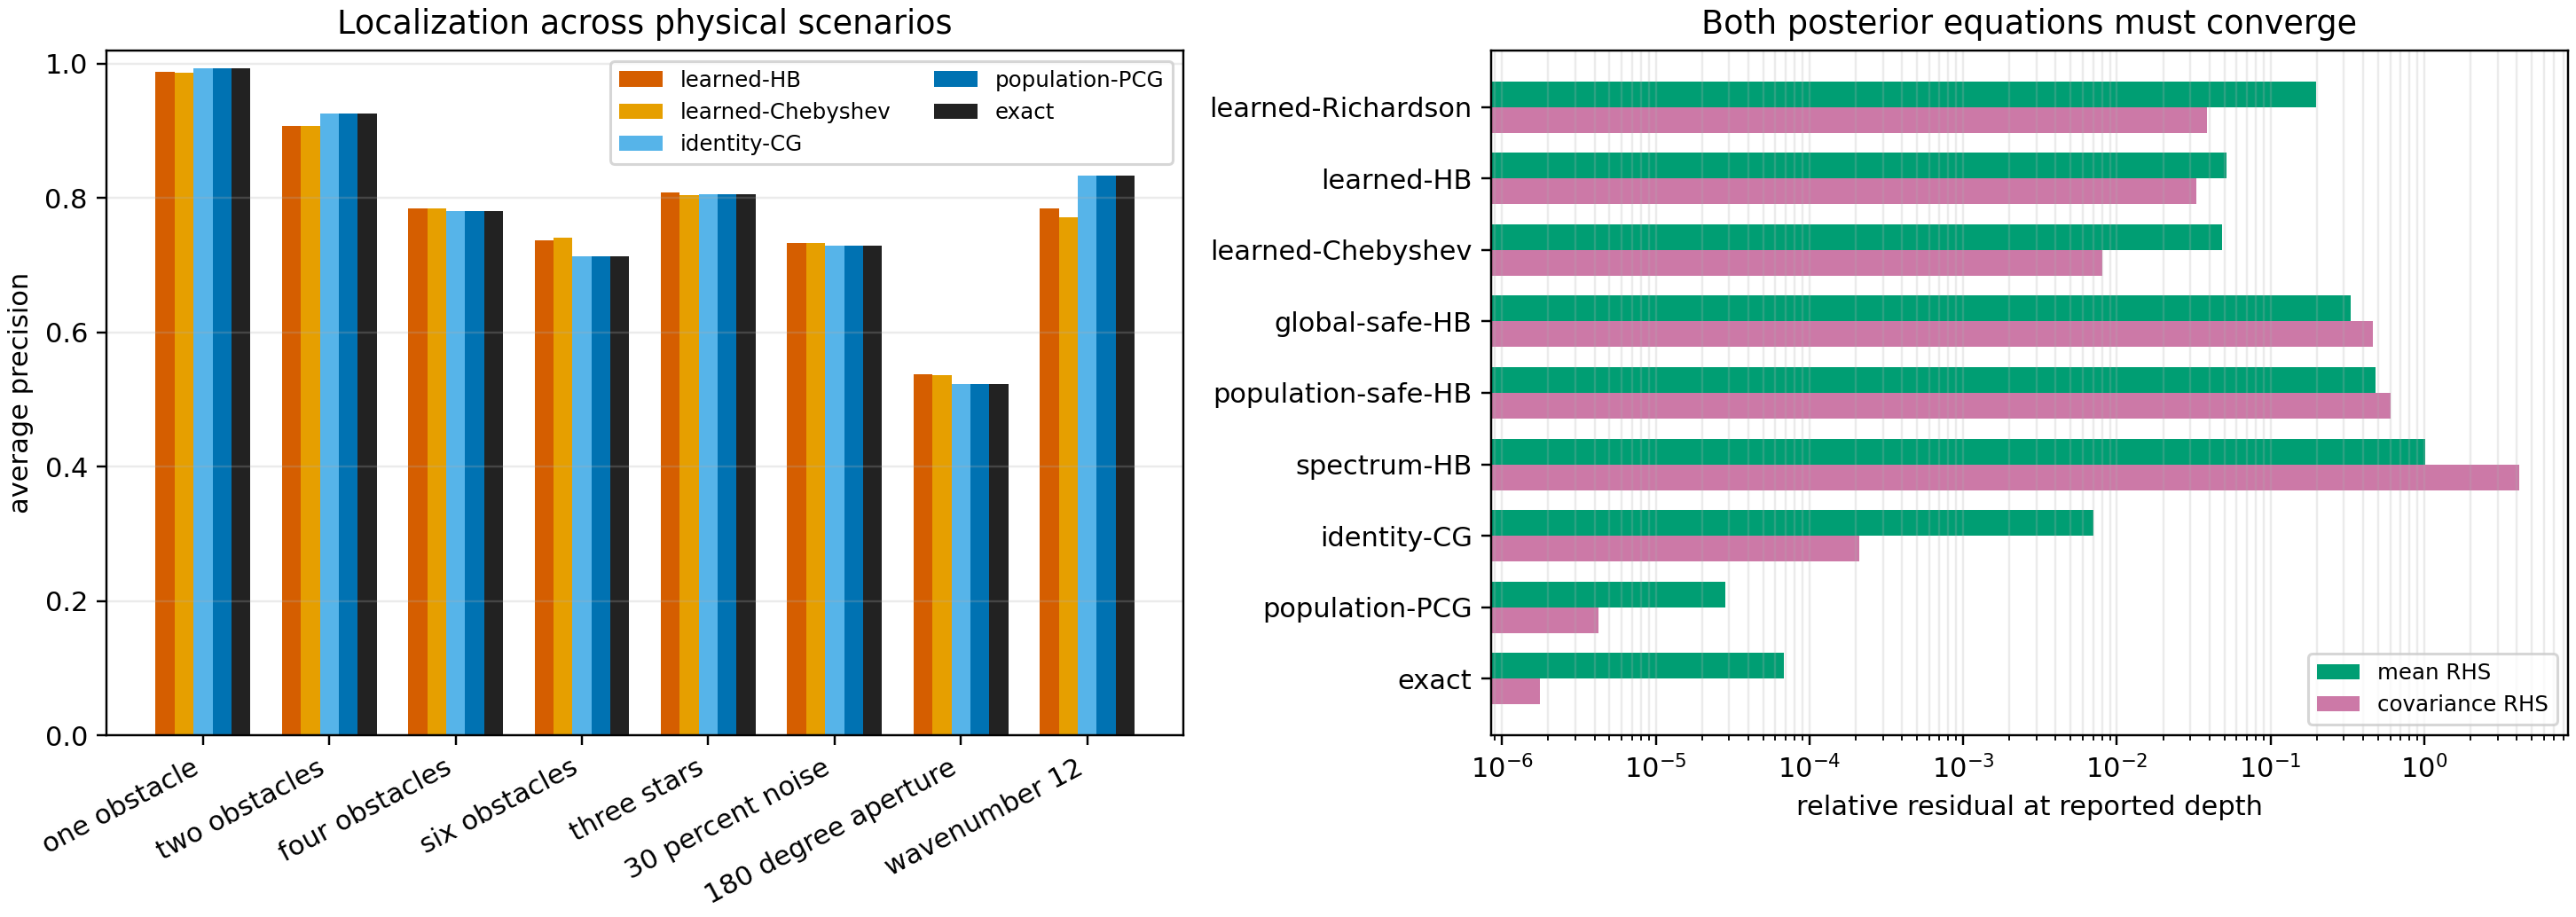
\includegraphics[width=\linewidth]{near_field_solver_summary.png}
\caption{Localization and the two distinct posterior residuals.  The exact
spectral HB diagnostic exposes the finite-depth transient.}
\end{figure}

\begin{figure}[t]
\centering
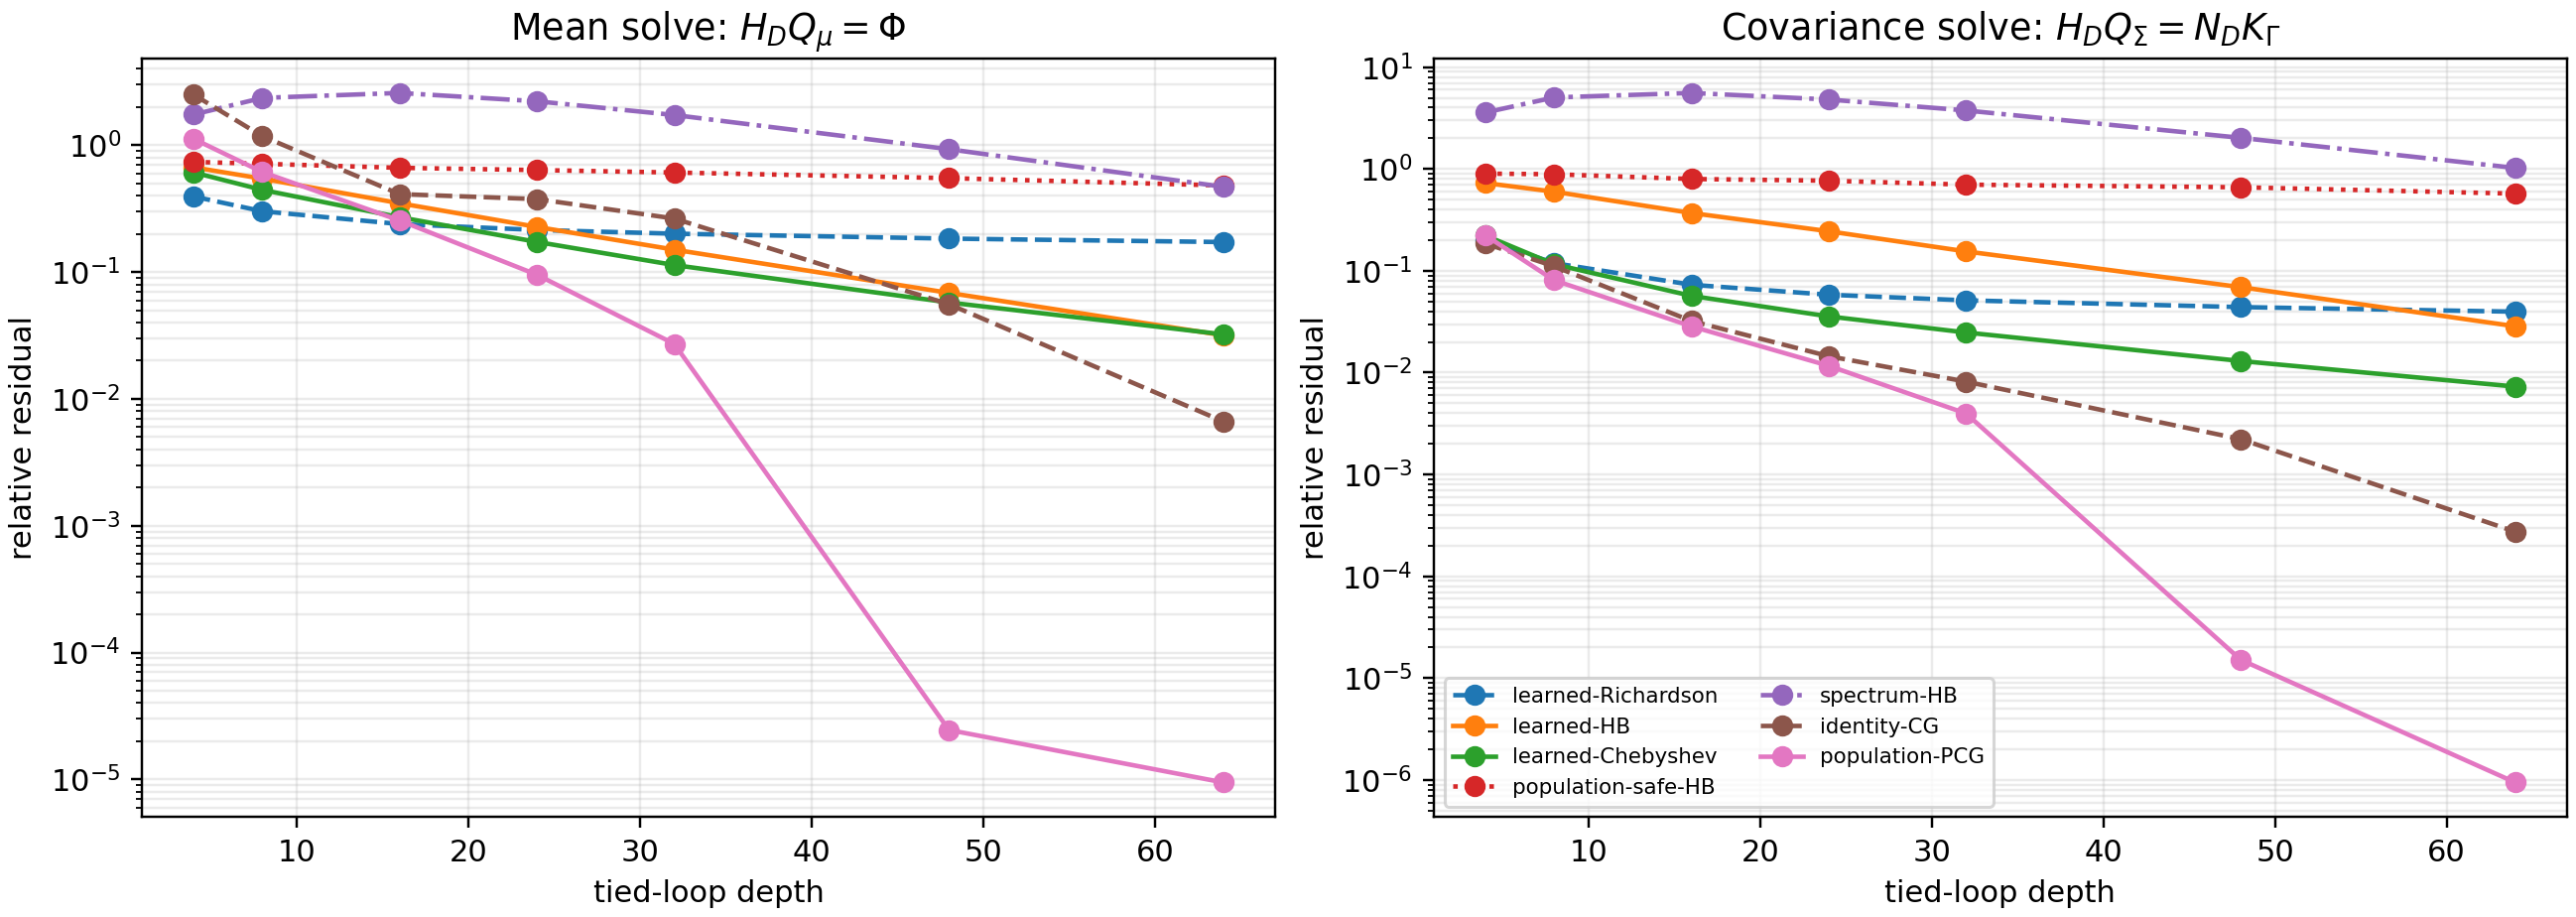
\includegraphics[width=0.96\linewidth]{near_field_depth_scaling.png}
\caption{Empirical depth laws on four-obstacle tasks.  PCG eventually enters
the small-residual regime; stationary methods remain condition-number limited.}
\end{figure}

The macro mean residuals are 5.135e-02
(learned HB), 4.847e-02 (learned
Chebyshev), 7.032e-03 (identity CG),
2.837e-05 (population PCG) and
6.791e-05 (direct).  The PCG/direct
mean-residual ratio is 0.42; PCG can attain a smaller measured
residual than the single-precision dense factorization, without changing the
underlying posterior.  Thus ``small'' must be defined relative to the
inferential target and floating-point precision.  Batched runtimes are
7.34 ms for learned HB,
10.74 ms for learned Chebyshev,
15.05 ms for identity CG,
16.44 ms for PCG and
1.91 ms for the small $24\times24$ dense reference
(medians across seeds).  At
this matrix size the direct solve is faster; recurrent scaling becomes relevant
only when structure, streaming, hardware reuse or much larger systems prohibit
factorization.

The equal-budget preconditioning test is direct: population-PCG reduces the
mean residual by a factor 247.91 and the covariance
residual by a factor 49.78 relative to identity
CG.  A factor above one is evidence that the in-context population transform
helps; a factor near or below one means that ordinary CG, rather than learned
conditioning, explains the convergence.

PCG and the direct solver have identical macro AP to four decimals
(0.7879) and visually indistinguishable
indicators.  Therefore the remaining blur in Figure~3 is not a solver-loss
problem.  It is the near-field point-spread/resolution limit of 24 channels at
one frequency: closely spaced components merge into a broad indicator even
after the linear system is solved.  More recurrent depth cannot sharpen that
map.  The relevant remedies are additional independent frequencies, more
source/receiver locations, a wider aperture, or an explicitly different
shape prior; the last option changes the Bayesian model and must not be hidden
inside the preconditioner.

\begin{figure}[t]
\centering
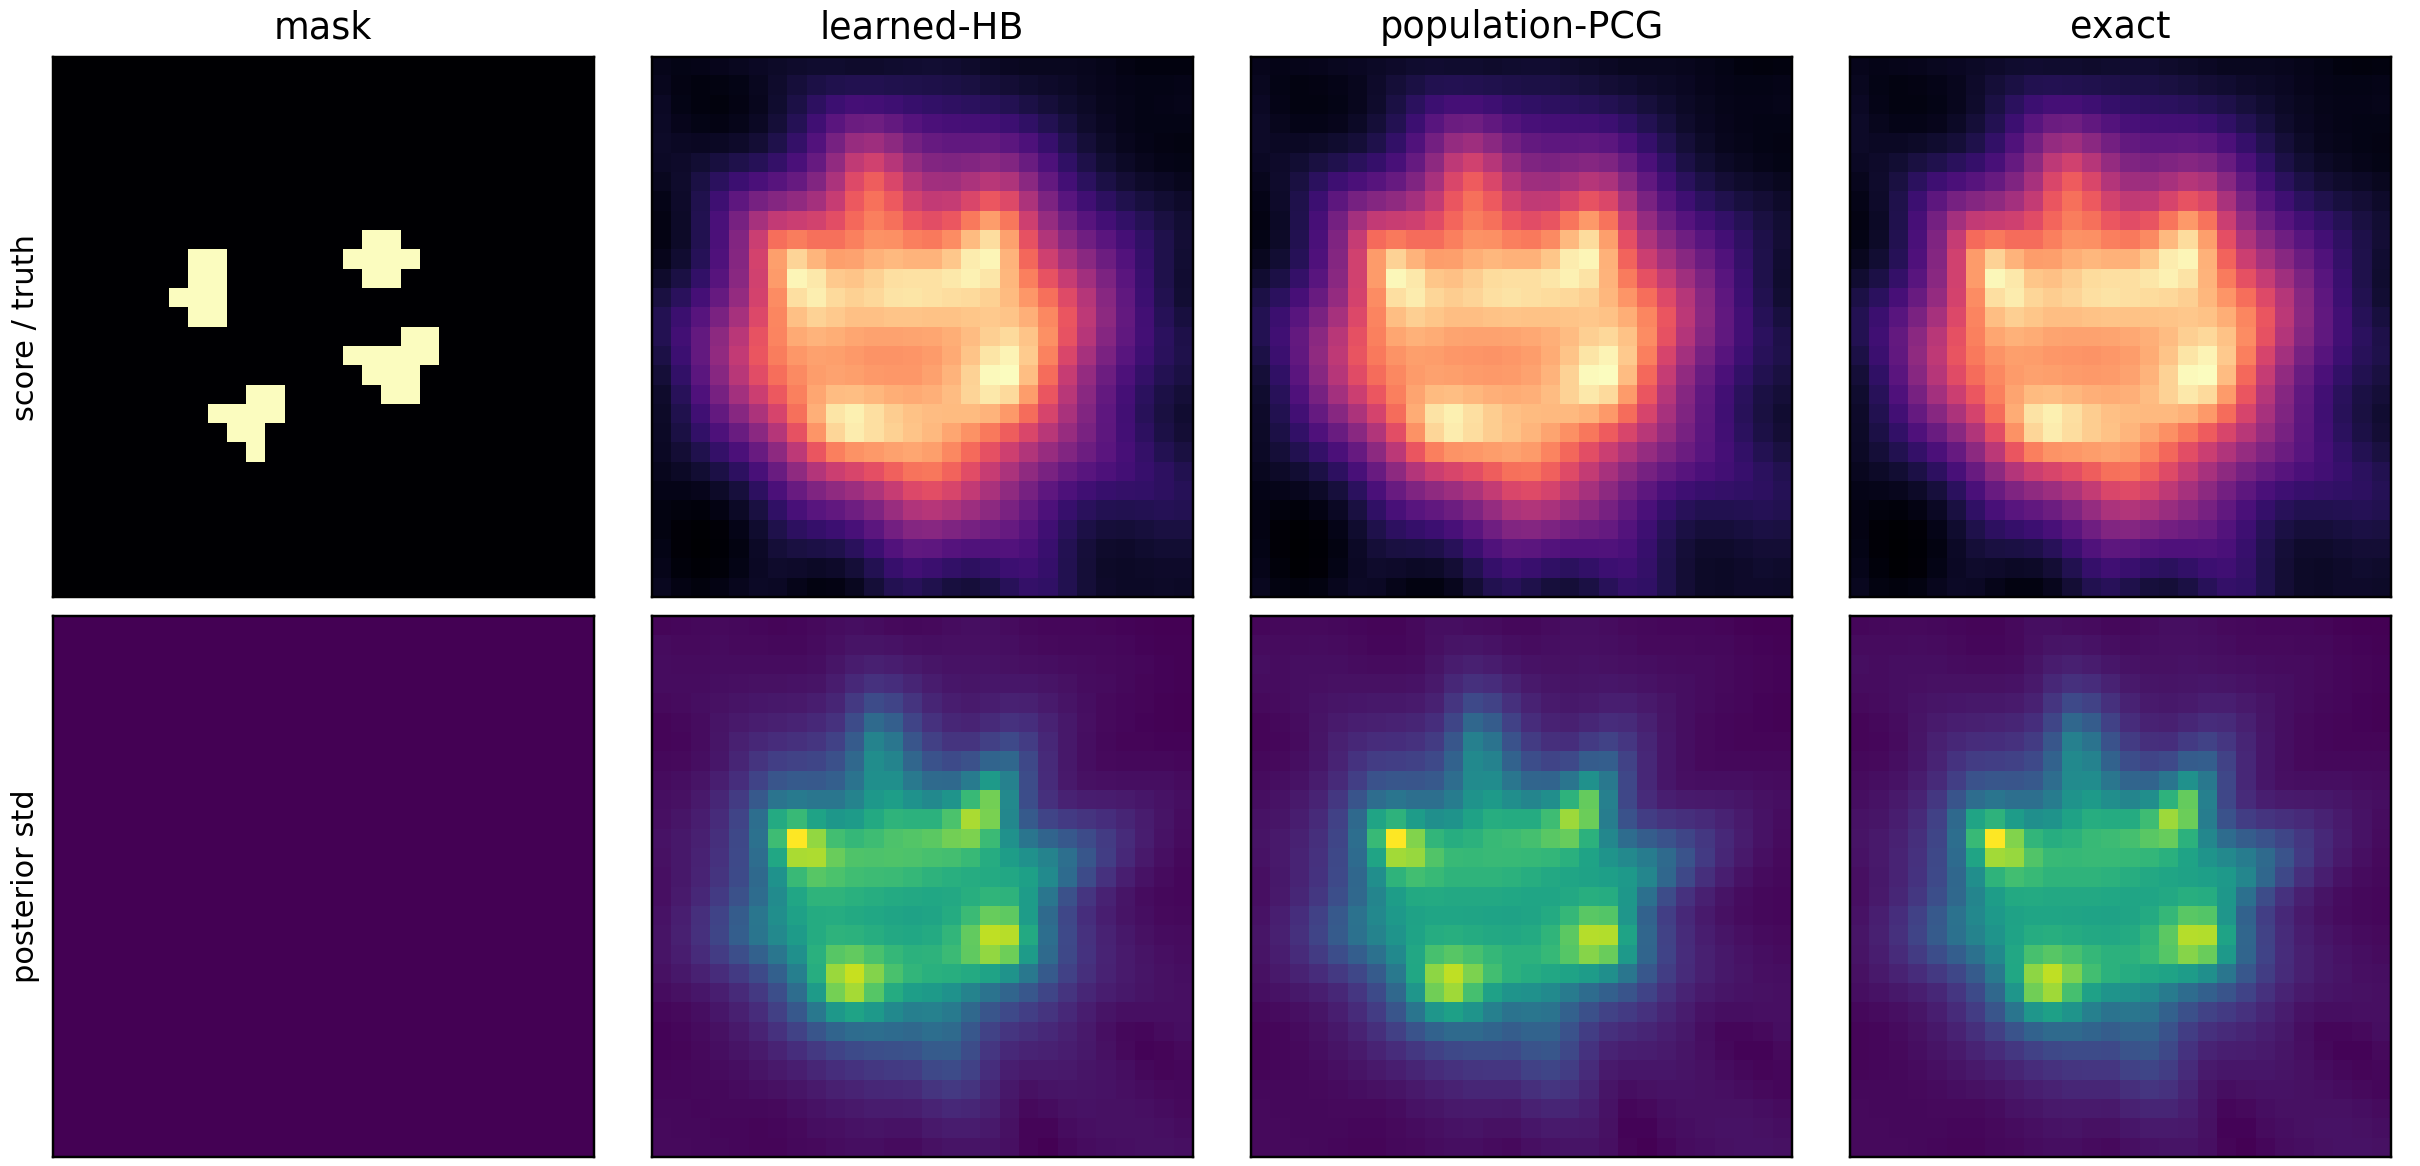
\includegraphics[width=0.96\linewidth]{near_field_reconstructions.png}
\caption{A held-out four-obstacle example.  The first row shows truth or
posterior score and the second row shows posterior score standard deviation.}
\end{figure}

\begin{figure}[t]
\centering
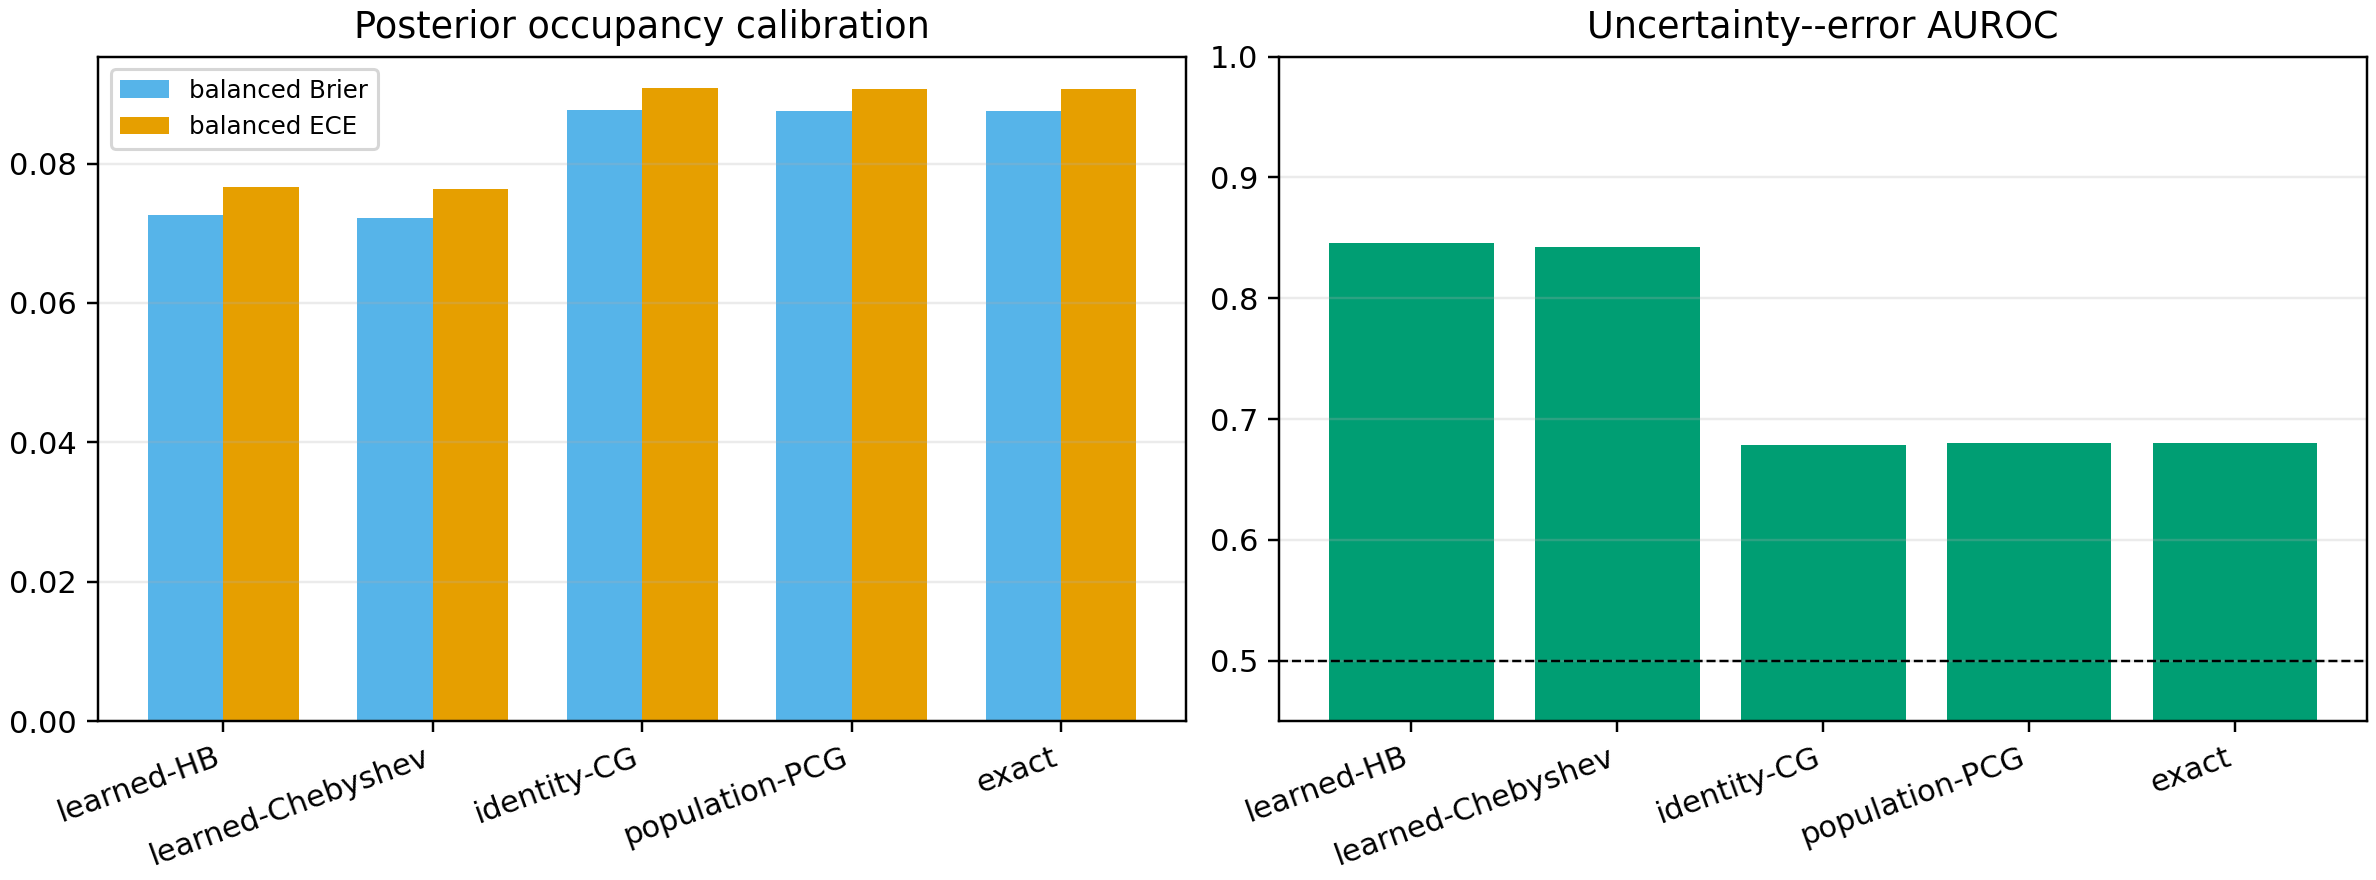
\includegraphics[width=0.88\linewidth]{near_field_uq_summary.png}
\caption{Bayesian UQ obtained from the second parallel recurrence.  Thresholds
are calibrated separately on training-distribution validation tasks.}
\end{figure}

The learned stationary loops have lower calibrated Brier scores and higher
uncertainty--error AUROC than the converged posterior.  This is an early-
stopping regularization effect, not evidence that an approximate covariance is
more faithful to the stated GP.  PCG/direct agreement is the appropriate test
of posterior correctness; calibration measures downstream occupancy utility.

\section{Interpretation and modelling recommendations}
The experiments support five conclusions.
\begin{enumerate}
\item The task is genuinely two-dimensional original near-field LSM: the input
is a complex multistatic response to several deterministic point sources.
\item The fixed softmax covariance is useful as prior geometry, but choosing it
cannot by itself erase the spectrum induced by the current obstacle.
\item Posterior mean and variance must be propagated together.  Solving only
$H_DQ_\mu=\Phi$ can produce attractive reconstructions with incorrect UQ.
\item Spectral endpoints contain signal, but exact asymptotic HB endpoints are
not the finite-depth optimum.  The controller should be trained against the
two residuals and audited against, rather than forced to equal, the spectrum.
\item For a genuinely small loss, use PCG or an $A_D$-equivariant polynomial
preconditioner and increase depth.  A larger generic MLP does not repair missing
task eigendirections.
\end{enumerate}

The next scientifically necessary step is to replace the MFS generator by an
independent high-order boundary-element solver and to test experimental near-
field data.  Until then, this is a controlled numerical validation, not a claim
of field-data performance.

\section{Reproducibility}
The code fixes all train/evaluation seeds, stores task-level tables and
checkpoints, and reports the exact scenario definitions in
\texttt{protocol.json}.  The principal model has
733,731 trainable parameters.  Source code and result
tables accompany this PDF.

\begin{thebibliography}{9}
\bibitem[Kang et~al.(2026)Kang, Lee, and Cheng]{kang2026}
G. Kang, C. J. Lee, and X. Cheng.
\newblock Transformers can learn posterior predictive distributions in-context.
\newblock \emph{arXiv:2605.26713}, 2026.

\bibitem[Kirsch and Grinberg(2008)]{kirsch2008}
A. Kirsch and N. Grinberg.
\newblock \emph{The Factorization Method for Inverse Problems}.
\newblock Oxford University Press, 2008.

\bibitem[Colton and Kress(2019)]{colton2019}
D. Colton and R. Kress.
\newblock \emph{Inverse Acoustic and Electromagnetic Scattering Theory}.
\newblock Springer, 4th edition, 2019.

\bibitem[Garnier et~al.(2022)Garnier, Haddar, and Montanelli]{montanelli2022}
J. Garnier, H. Haddar, and H. Montanelli.
\newblock The linear sampling method for random sources.
\newblock \emph{arXiv:2210.15560}, 2022.

\bibitem[Garnier et~al.(2024)Garnier, Haddar, and Montanelli]{montanelli2024}
J. Garnier, H. Haddar, and H. Montanelli.
\newblock The linear sampling method for data generated by small random scatterers.
\newblock \emph{arXiv:2403.19482}, 2024.

\bibitem[Polyak(1964)]{polyak1964}
B. T. Polyak.
\newblock Some methods of speeding up the convergence of iteration methods.
\newblock \emph{USSR Computational Mathematics and Mathematical Physics}, 1964.
\end{thebibliography}
\end{document}
